\documentclass{beamer}
\usetheme[compressed]{Singapore}
\useinnertheme{circles}
%\usetheme{Montpellier}
\usepackage[italian]{babel}
\setbeamercolor{background canvas}{bg=background}
\setbeamercolor{section in toc}{fg=template}
\setbeamercolor{subsection in toc}{fg=black}
\setbeamerfont{section in toc}{series=\bfseries,size=\normalsize}
\definecolor{background}{RGB}{255, 255, 255}
\definecolor{royalblue3}{RGB}{58,95,205}
\definecolor{giallo}{RGB}{197, 151, 0}
%\definecolor{template}{RGB}{54, 114, 89}
\definecolor{template}{RGB}{181, 18, 27}
\setbeamercolor{section in head/foot}{fg=white, bg=template}
\setbeamercolor{subsection in head/foot}{fg=template, bg=template!20}
\setbeamercolor{subsection in head/foot}{fg=template, bg=template!20}
\setbeamercolor{frametitle}{fg=template, bg = white}
\setbeamercolor{title}{bg = white, fg=template}
\setbeamercolor{author in head/foot}{bg=template, fg=white}
\setbeamercolor{title in head/foot}{bg=template!40, fg=template}
\setbeamercolor{date in head/foot}{bg=template!20, fg=template}
\setbeamercolor{item}{fg=template!20}
\setbeamercolor{caption name}{fg=template}
\usepackage{tikz}
\usetikzlibrary{shapes}
\usetikzlibrary{plotmarks}
\usetikzlibrary{mindmap,calc,patterns,decorations.pathmorphing,decorations.markings, arrows, shapes.arrows, shapes, backgrounds,positioning,shadows.blur, positioning, fit}
\usepackage{multirow}
\usepackage{tabularx}
\usepackage{setspace}
\usepackage{booktabs}
\usepackage{tikz}
\usepackage{mathtools}
\usepackage{atbegshi}
\usepackage{amsmath}
%\usetikzlibrary{arrows,shapes}
\usepackage[absolute,overlay]{textpos}
\newcommand\Factor{1.2}

\tikzset{type1/.style={circle, fill=template},
	type2/.style={circle, fill=red},
		type3/.style={circle, fill=olive},
			type4/.style={circle, fill=cyan},
				type5/.style={circle, fill=giallo},
					type6/.style={circle, fill=template},
	info/.style = {rectangle, rounded corners, minimum width=2.5cm, minimum height=0.1cm, text centered, draw=black,  text width=2.5cm},
	stat/.style = {rectangle, rounded corners, minimum width=2.5cm, minimum height=0.1cm, text centered, draw=white,  text width=2.5cm}
}

\AtBeginSection[]
{
	\begin{frame}
		\tableofcontents[currentsection,currentsubsection]
	\end{frame}
}  

\AtBeginSubsection[]
{
	\begin{frame}
		\tableofcontents[currentsection,currentsubsection]
	\end{frame}
}  

\AtBeginSubsubsection[]
{
	\begin{frame}
		\tableofcontents[currentsection,currentsubsection]
	\end{frame}
}  

\newcommand{\tstar}[5]{% inner radius, outer radius, tips, rot angle, options
	\pgfmathsetmacro{\starangle}{360/#3}
	\draw[#5] (#4:#1)
	\foreach \x in {1,...,#3}
	{ -- (#4+\x*\starangle-\starangle/2:#2) -- (#4+\x*\starangle:#1)
	}
	-- cycle;
}

\newcommand{\ngram}[4]{% outer radius, tips, rot angle, options
	\pgfmathsetmacro{\starangle}{360/#2}
	\pgfmathsetmacro{\innerradius}{#1*sin(90-\starangle)/sin(90+\starangle/2)}
	\tstar{\innerradius}{#1}{#2}{#3}{#4}
}

 \tikzset{
	invisible/.style={opacity=0},
	visible on/.style={alt={#1{}{invisible}}},
	alt/.code args={<#1>#2#3}{%
		\alt<#1>{\pgfkeysalso{#2}}{\pgfkeysalso{#3}} % \pgfkeysalso doesn't change the path
	},
	every overlay node/.style={
		%draw=black,fill=white,rounded corners,
		anchor=north west, inner sep=0pt,
	},
}

\def\tikzoverlay{%
	\tikz[remember picture, overlay]\node[every overlay node]
}%

%\setbeamertemplate{section page}
%{
%	\begingroup
%	\begin{beamercolorbox}[sep=12pt,center]{section title}
%		\usebeamerfont{section title}\insertsection\par
%	\end{beamercolorbox}
%	\endgroup
%}




\title[Questionnaires and Beyond]{Questionnaires and beyond: \\ The Rasch model
}
\institute[]{Padova}
\author[]{\texorpdfstring{Ottavia M. Epifania\newline\url{ottavia.epifania@unipd.it} \newline Univerisity of  Padova \newline Catholic University of the Sacred Heart}{Author}}
\date{Antani convegno AIP}
\titlegraphic{%
	
\includegraphics[width=1.8cm,height=1.8cm,keepaspectratio]{unipd.png}%\hspace*{9.75cm}~%
	
\includegraphics[width=2.5cm,height=2.5cm,keepaspectratio]{psicostat.png}%
	
\includegraphics[width=1.8cm,height=1.8cm,keepaspectratio]{unicatt.png}%
}
\begin{document}
\begin{frame}[plain]
    \maketitle
\end{frame}

\section{The intuition}

\begin{frame}
\tikzoverlay (math) at (1.5cm,2.0cm) {%
	\begin{minipage}{.60\textwidth}
\begin{columns}[T]
		
	\begin{column}{.50\linewidth}
		\centering \textbf{Q1}
		\begin{equation*}
			4 + 5 = ?
		\end{equation*}
	\end{column}

	\begin{column}{.50\linewidth}
		\centering \textbf{Q2}
		\begin{equation*}
			\dfrac{3}{2} + \dfrac{5}{4} = ?
		\end{equation*}
\end{column}
\end{columns}
	\end{minipage}
};
\onslide<2->
\tikzoverlay (math1) at (1.3cm,0.5cm) {%
	\begin{minipage}{.60\textwidth}
		\begin{columns}[T]
			
			\begin{column}{.50\linewidth}
				\begin{equation*}
					d_{q1}
				\end{equation*}
			\end{column}
			\begin{column}{.50\linewidth}
				\begin{equation*}
				d_{q2}
			\end{equation*}
			\end{column}
		\end{columns}
	\end{minipage}
};
\onslide<3->
\tikzoverlay (bart) at (-0.8cm,2.2cm) {%
	\begin{minipage}{.20\textwidth}
		
		\begin{figure}
			\centering
			
\includegraphics[width=\linewidth]{bart.png}
		\end{figure}
	\end{minipage}
};
\tikzoverlay (bart1) at (-0.8cm,-1.3cm) {%
	\begin{minipage}{.20\textwidth}
		\centering
		$A_\text{Bart}$

	\end{minipage}
};
\tikzoverlay (lisa) at (8.5cm,1.5cm) {%
	\begin{minipage}{.20\textwidth}
		\begin{figure}
			\centering
			
\includegraphics[width=\linewidth]{lisa.png}
		\end{figure}
	\end{minipage}
};

\tikzoverlay (lisa1) at (9.2cm,-0.5cm) {%
	\begin{minipage}{.20\textwidth}
				\centering
		$A_\text{Lisa}$
		
	\end{minipage}
};
\tikzoverlay (eq) at (0.3cm, -1.5cm){
\begin{minipage}{.30\linewidth}
	\begin{equation}
		\dfrac{A_p}{d_i}
	\end{equation}
\centering
\vspace{3mm}
$> 1$ if $A_p > d_i$

$< 1$ if $A_p < d_i$
\end{minipage}
};
\tikzoverlay (eq1) at (5.3cm, -1.5cm){
	\begin{minipage}{.50\linewidth}
		\begin{equation}
			P(X_{pi} = 1) = \dfrac{\dfrac{A_p}{d_i}}{1 + \dfrac{A_p}{d_i}}
		\end{equation}
	\end{minipage}
};
\end{frame}

\section{The model}
\begin{frame}
\begin{figure}
	\centering
	
\includegraphics[width=0.5\linewidth]{later}
\end{figure}
\begin{columns}[T]
	\begin{column}{.5\linewidth}
		\centering
		$ln(A_p) = \beta_p$
	\end{column}
	\begin{column}{.5\linewidth}
	\centering
	$ln(d_i) = \delta_i$
\end{column}
\end{columns}

\vspace{3mm}
\begin{equation}
P(X_{vi}|\beta_p, \delta_i) = \dfrac{exp(\beta_p - \delta_i)}{1 + exp(\beta_p - \delta_i)}
\end{equation}
\end{frame}

\begin{frame}

	\begin{overprint}
		\centering
	\onslide<1>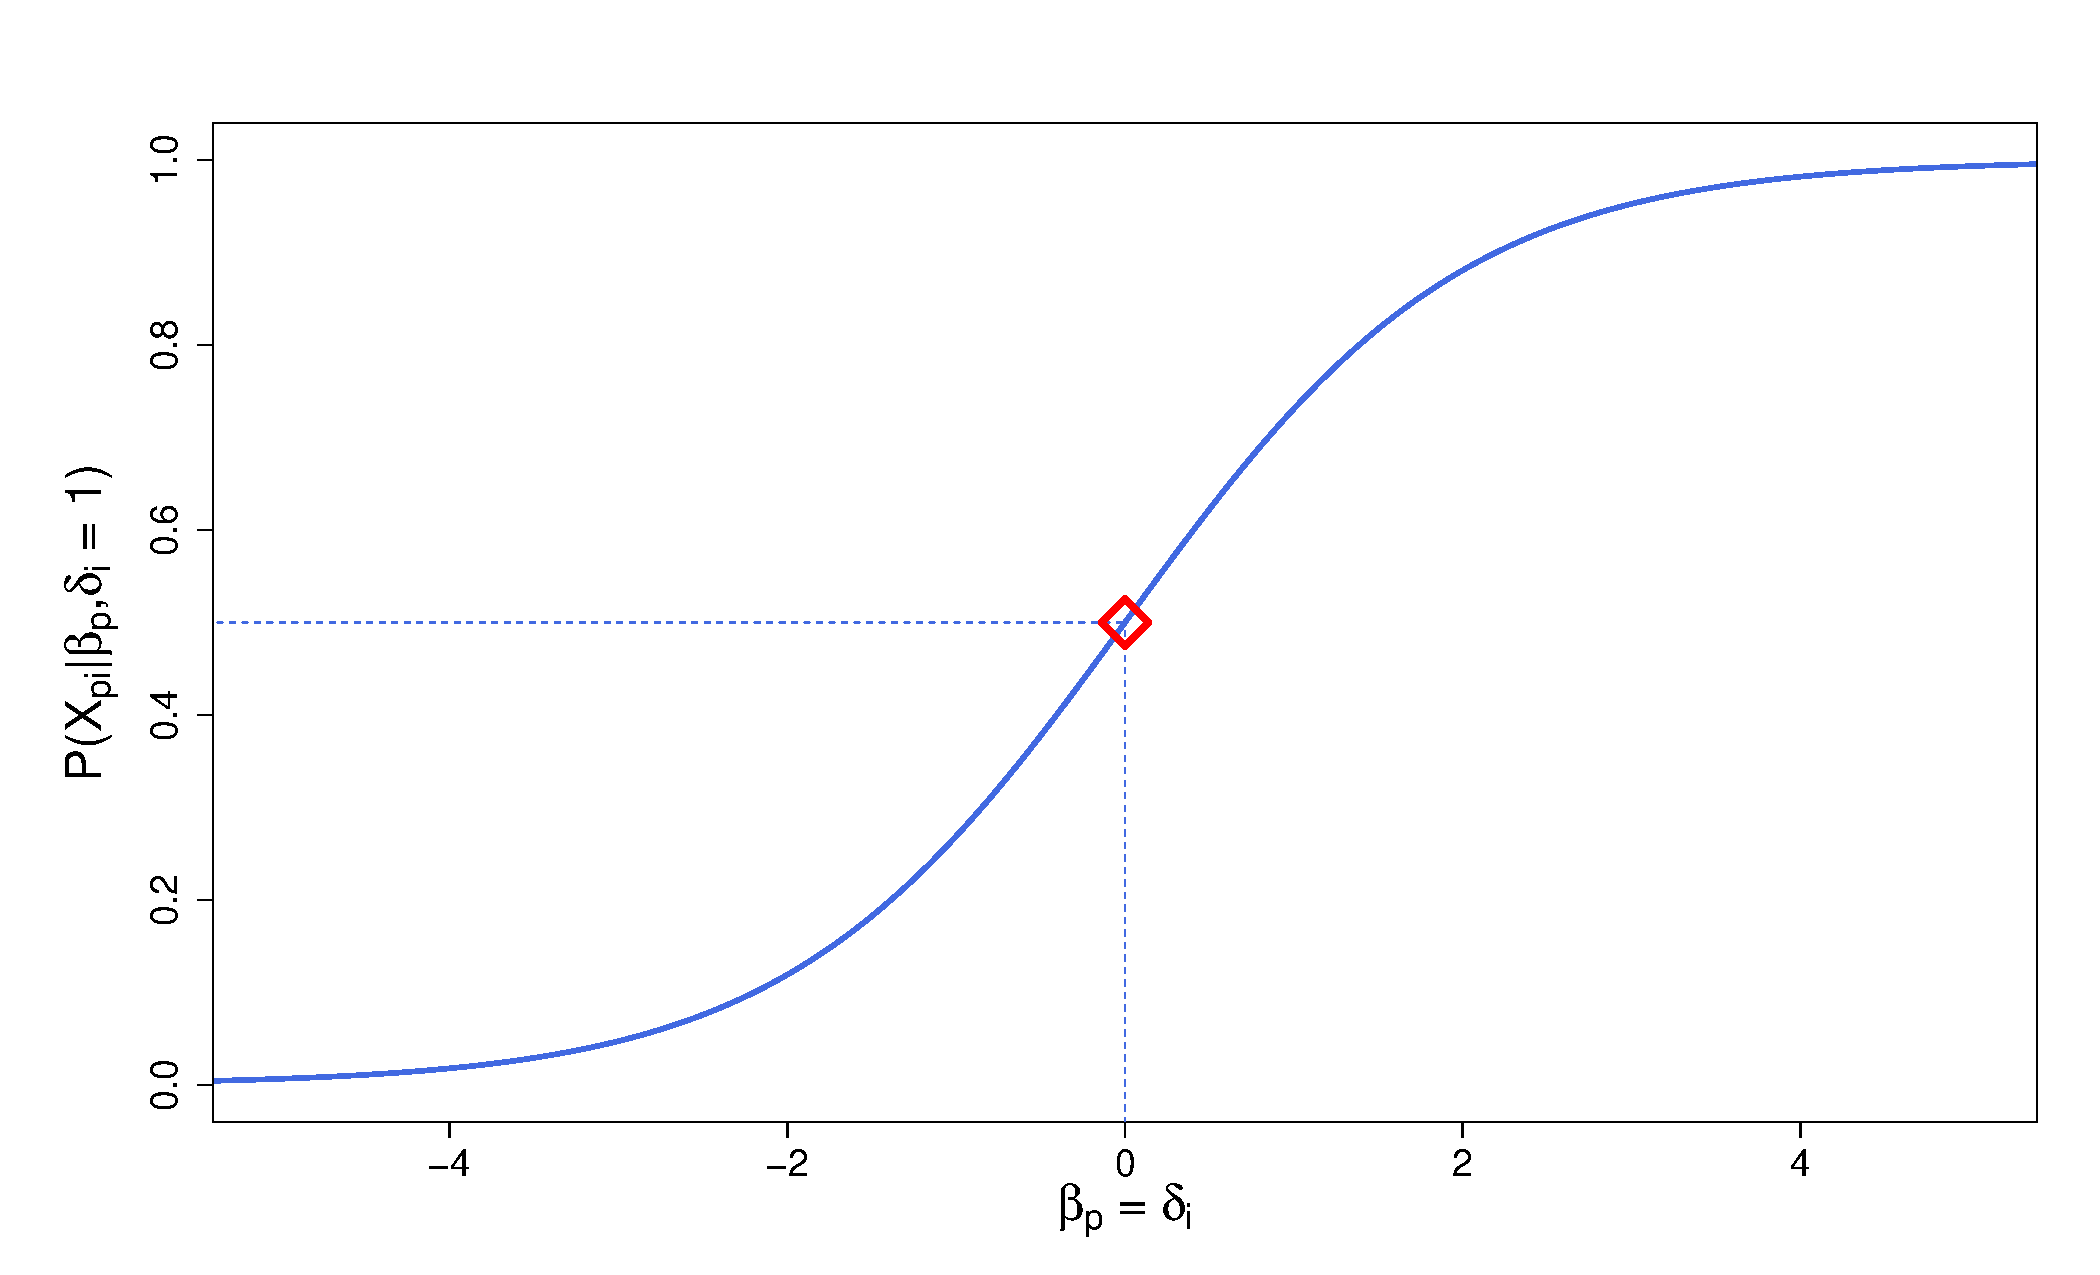
\includegraphics[width=\linewidth]{base.pdf}
	\onslide<2>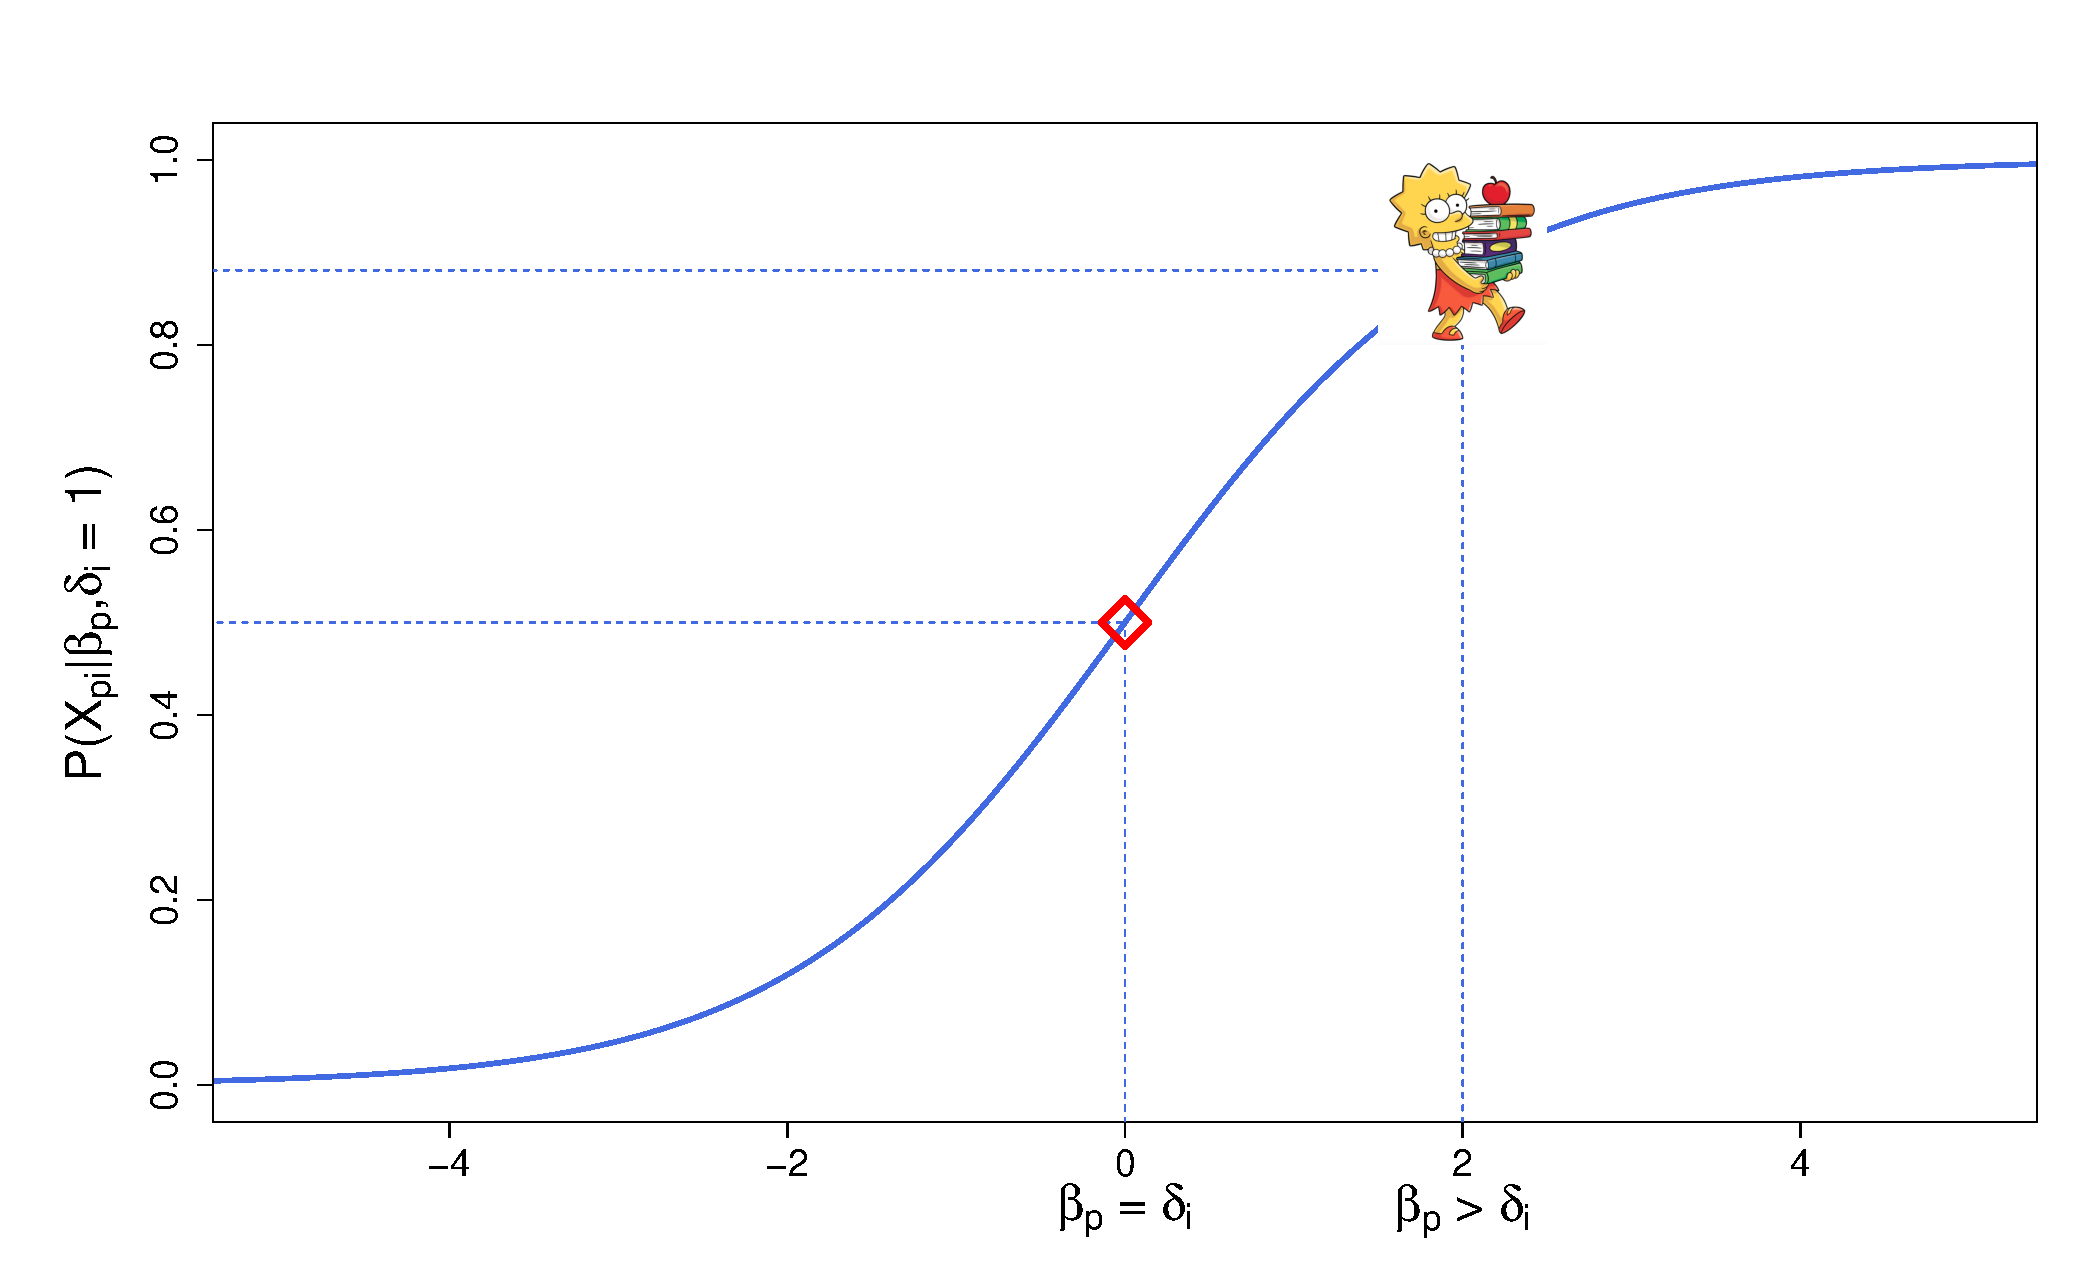
\includegraphics[width=\linewidth]{lisa.pdf}
	\onslide<3>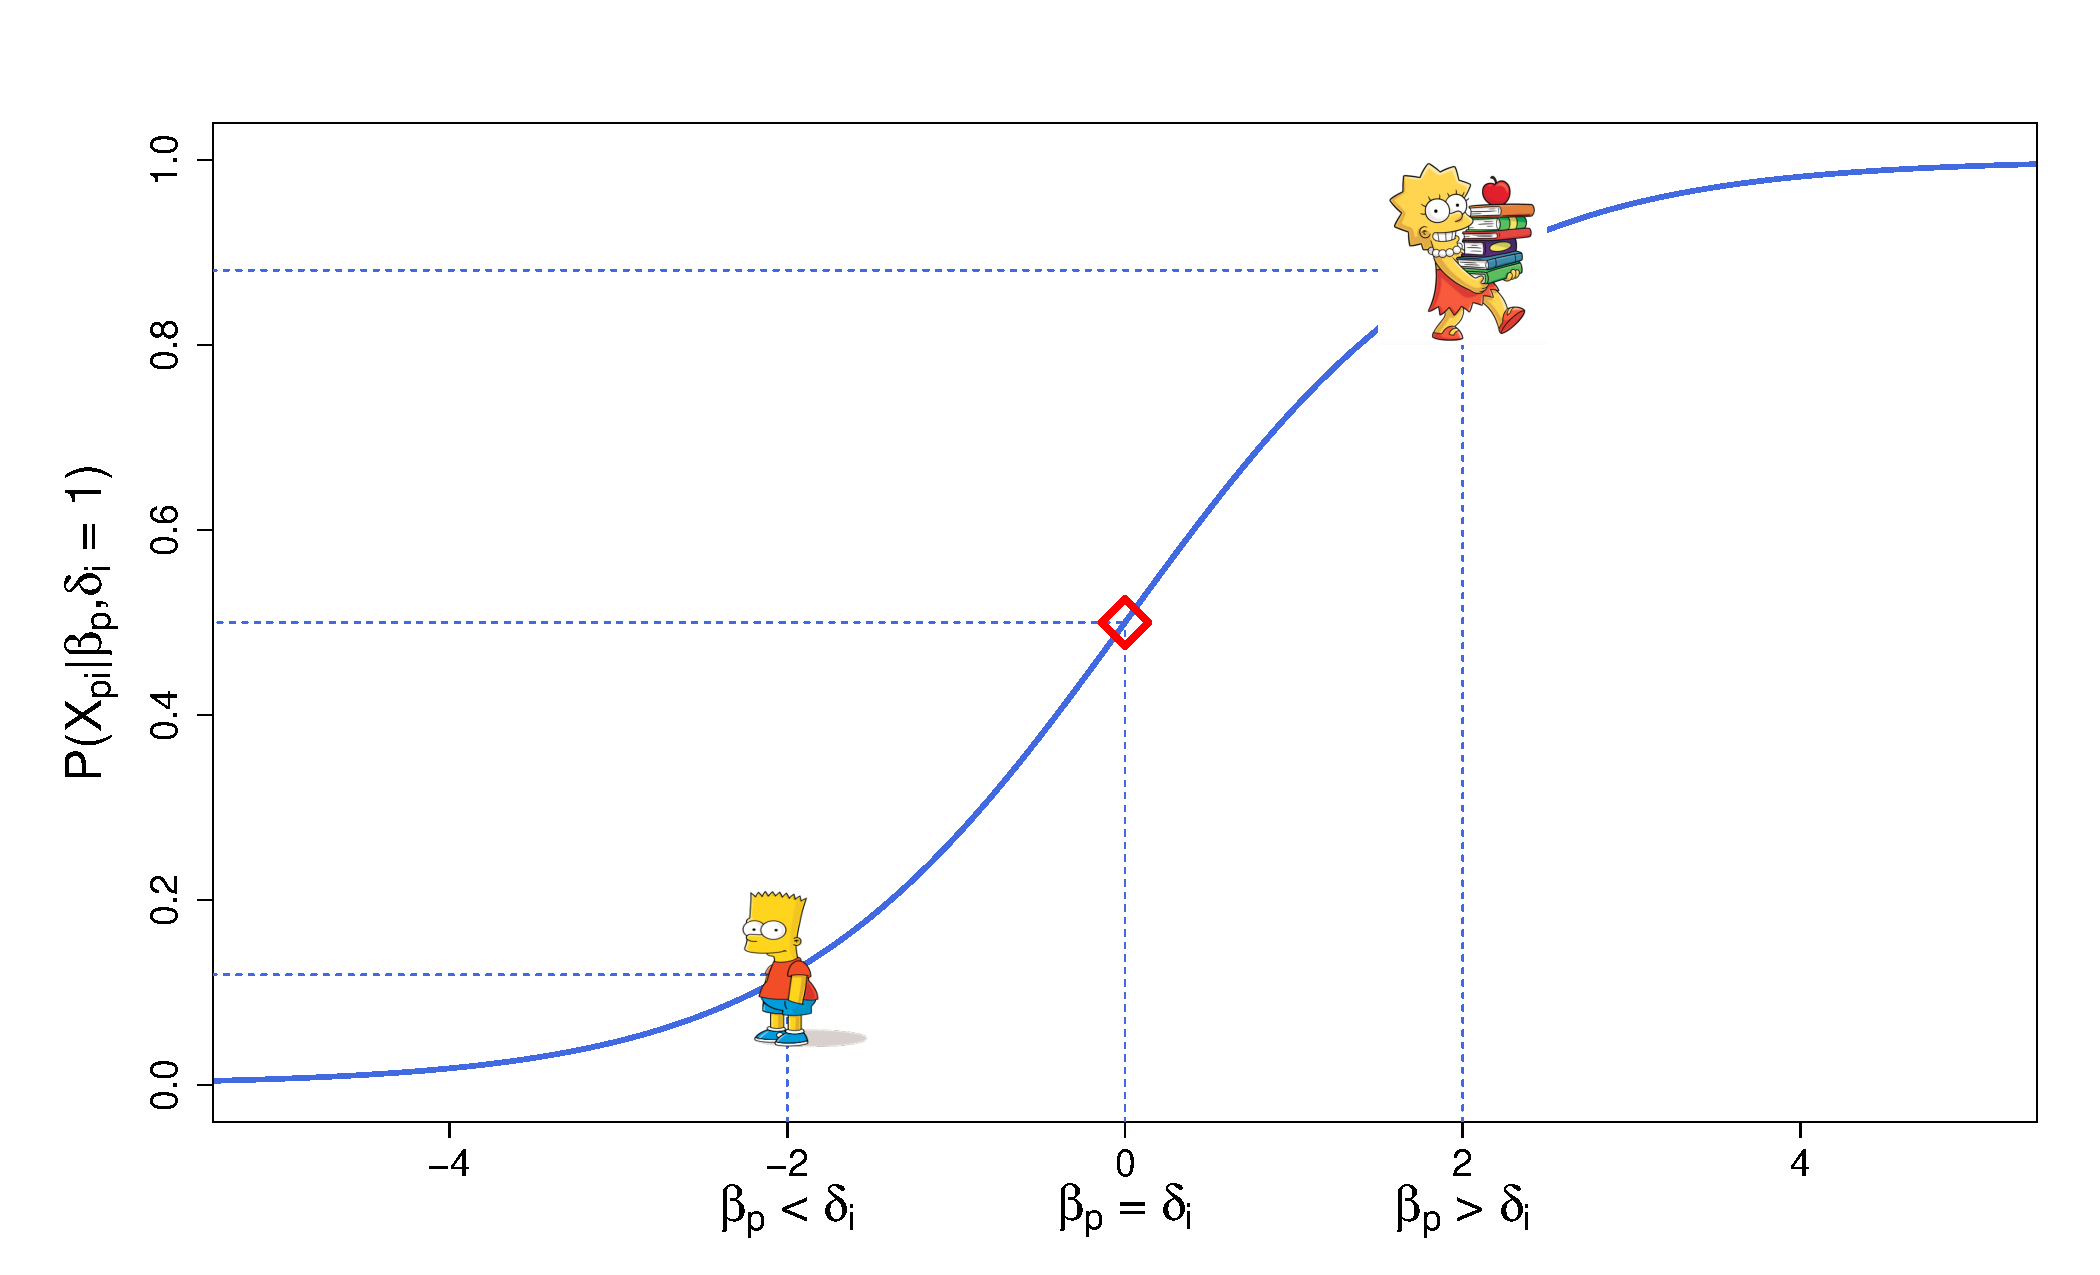
\includegraphics[width=\linewidth]{bart.pdf}
\end{overprint}
\end{frame}

\section{Wait...}

\section{Beyond}

\begin{frame}
	\begin{tikzpicture}
		\node (a) [type1, xshift=-3cm] {};
		\node (b) [type2, right of=a, xshift=0.5cm]{};
\node (c) [type3, right of=b, xshift=0.5cm]{};
\node (d) [type4, right of=c, xshift=0.5cm]{};
\node (e) [type5, right of=d, xshift=0.5cm]{};
\node (f) [type6, right of=e, xshift=0.5cm]{};
\node (pop)[info, right of =f , xshift=1.5cm] {Popolazione};
\onslide<2->
	\node[draw=red,fit=(a) (b) ,inner sep=0.8ex,ellipse] (c1) {};
\node[draw=black,fit=(b) (c) ,inner sep=0.5ex,ellipse] (c2) {};
\node[draw=template,fit=(c) (d) ,inner sep=0.8ex,ellipse] (c3) {};
	\node[draw=cyan,fit=(d) (e) ,inner sep=0.5ex,ellipse] (c4) {};	
	\node[draw=olive,fit=(e) (f) ,inner sep=0.8ex,ellipse] (c5) {};
		
\node (g1a) [type1,below of=c1, xshift=-0.8cm, yshift=-0.5cm] {};
\node (g1b) [type2,right of=g1a, xshift=-0.3cm] {};
		\node[draw = black, fit = (g1a) (g1b), rectangle] (g1) {};
		
		\node (g2a) [type2,right of=g1b, xshift=0.15cm] {};
		\node (g2b) [type3,right of=g2a, xshift=-0.3cm] {};
		\node[draw = black, fit = (g2a) (g2b), rectangle] (g2) {};
		
				
		\node (g3a) [type3,right of=g2b, xshift=0.15cm] {};
		\node (g3b) [type4,right of=g3a, xshift=-0.3cm] {};
		\node[draw = black, fit = (g3a) (g3b), rectangle] (g3) {};
		
				\node (g4a) [type4,right of=g3b, xshift=0.15cm] {};
		\node (g4b) [type5,right of=g4a, xshift=-0.3cm] {};
		\node[draw = black, fit = (g4a) (g4b), rectangle] (g4) {};
		
					\node (g5a) [type5,right of=g4b, xshift=0.15cm] {};
		\node (g5b) [type6,right of=g5a, xshift=-0.3cm] {};
		\node[draw = black, fit = (g5a) (g5b), rectangle] (g5) {};
		
		\node (campione) [info, right of=g5, xshift=1.5cm] {Campione};

		\draw[thick,->,>=stealth, red] (c1) edge  (g1);
		\draw[thick,->,>=stealth, black] (c2) edge  (g2);
		\draw[thick,->,>=stealth, template] (c3) edge  (g3);
		\draw[thick,->,>=stealth, cyan] (c4) edge  (g4);
		\draw[thick,->,>=stealth, giallo] (c5) edge  (g5);
			\onslide<3->	
		\node (m1) [stat, below of= g1, yshift=-1cm] {\color{red}$M_1$};
			\node (m2) [stat, below of= g2, yshift=-1cm] {\color{black}$M_2$};
	\node (m3) [stat, below of= g3, yshift=-1cm] {\color{template}$M_3$};
		\node (m4) [stat, below of= g4, yshift=-1cm] {\color{cyan}$M_4$};
			\node (m5) [stat, below of= g5, yshift=-1cm] {\color{giallo}$M_5$};
			
			\draw[thick,->,>=stealth] (g1) edge  (m1);
			\draw[thick,->,>=stealth] (g2) edge  (m2);
			\draw[thick,->,>=stealth] (g3) edge  (m3);
			\draw[thick,->,>=stealth] (g4) edge  (m4);
			\draw[thick,->,>=stealth] (g5) edge  (m5);
			
			\node (statistica) [info, right of= m5, xshift = 1cm] {Statistica};
			
			\onslide<4->
			\node (mediaGen) [info, below of= m3, yshift= -1cm] {$\mu_{\bar{X}} = \mu$};
				\node (statistica) [info, below of= statistica,  yshift= -1cm] {Distribuzione campionaria della media};
				
							\draw[thick,->,>=stealth] (m1) edge  (mediaGen);
				\draw[thick,->,>=stealth] (m2) edge  (mediaGen);
				\draw[thick,->,>=stealth] (m3) edge  (mediaGen);
				\draw[thick,->,>=stealth] (m4) edge  (mediaGen);
				\draw[thick,->,>=stealth] (m5) edge  (mediaGen);
	\end{tikzpicture}

\onslide<2->
\begin{alertblock}{N.B.:}
	
	Sono illustrati solo alcuni dei possibili $k$ campioni 
\end{alertblock}
\end{frame}




\end{document}
